\documentclass[../mathNotesPreamble]{subfiles}

\begin{document}
%  \relscale{1.4} %TODO
  \section{3.3: Summaries for Skewed Distributions}
  \begin{defn*}
    The \textbf{median} of a sample of data is the middle value when the data is sorted from smallest to largest. If the set contains an
    \begin{itemize}
      \item odd number of observed values, the median is the middle observed value.
      \item even number of observed values, the median is the average of the two middle observed values.
    \end{itemize}
    The median is the preferred measure of center when the data is skewed since about 50\% of the observations lie below and above the median.
  \end{defn*}
  
  \begin{ex*}
    The prices of 1 gallon of regular gas at 12 service stations near the downtown area of Austin, TX, were as follows one winter day in 2018:
    \vspace*{\baselineskip}
    
    \noindent
    \begin{minipage}{0.4\linewidth}
      \begin{center}
        \begin{tabular}{@{}*{4}{c}@{}}\toprule
          \$2.19 & \$2.19 & \$2.39 & \$2.19 \\
          \$2.24 & \$2.39 & \$2.27 & \$2.29 \\
          \$2.17 & \$2.29 & \$2.30 & \$2.29 \\\bottomrule
        \end{tabular}
      \end{center}
    \end{minipage}\hspace*{\stretch{1}}
    \begin{minipage}{0.6\linewidth}
      \centering
      \begin{tikzpicture}
        \begin{axis}[
          axis lines=center,
          axis line style={black,->},
          xmin=2.14, xmax=2.41,
          ymin=0,
          ymajorticks=false,
          width=0.9\linewidth,
          height=0.33\linewidth,
          ticklabel style={font=\normalsize,inner sep=0.5pt,fill=white,opacity=1.0, text opacity=1}]
            \foreach \price/\freq in {
              2.17/1,
              2.19/3,
              2.24/1,
              2.27/1,
              2.29/3,
              2.3/1,
              2.39/2
              }{
              \foreach \x in {1,...,\freq}
                \addplot[soldot, mark size=2pt] coordinates{(\price,\x)};
              }
        \end{axis}
      \end{tikzpicture}
    \end{minipage}
  \end{ex*}
  \noindent Find the median price for a gallon of gas and interpret the value.
  \pagebreak
  
  \begin{ex*}
    Below are the percentages of fat for some brands of sliced turkey:\\
    
    \noindent
    \begin{minipage}{0.375\linewidth}
      \[14, 10, 20, 20, 40, 20, 10, 10, 20, 50, 10\]
    \end{minipage}
    \hspace*{\stretch{1}}%
    \begin{minipage}{0.6\linewidth}
      \centering
      \begin{tikzpicture}
        \begin{axis}[
          axis lines=center,
          axis line style={black,->},
          xmin=6, xmax=54,
          ymin=0,
          ymajorticks=false,
          width=0.9\linewidth,
          height=0.33\linewidth,
          ticklabel style={font=\normalsize,inner sep=0.5pt,fill=white,opacity=1.0, text opacity=1}]
            \foreach \price/\freq in {
              10/4,
              14/1,
              20/4,
              40/1,
              50/1
              }{
              \foreach \x in {1,...,\freq}
                \addplot[soldot, mark size=2pt] coordinates{(\price,\x)};
              }
        \end{axis}
      \end{tikzpicture}
    \end{minipage}
    \vspace*{\baselineskip}
      
    \noindent
    Find the median percentage of fat and interpret the value.
  \end{ex*}
  \pagebreak
  
  \begin{defn*}
    \begin{itemize}
      \item The \textbf{range} is the difference between the maximum and minimum values:
        \[\textnormal{Range}=\textnormal{maximum}-\textnormal{minimum}\]
      \item The \textbf{quartiles} divide the data into quarters.
      \item The \textbf{interquartile range (IQR)} indicates approximately how much space the middle 50\% of the data occupy.
    \end{itemize}
  \end{defn*}
  \begin{ex*}
    The dotplot below shows the distribution of weights for a class of introductory statistics students.
    \begin{itemize}
      \item Label each line
      \item Compute the IQR
    \end{itemize}
  \end{ex*}
  \vspace*{\stretch{1}}
  \begin{center}
    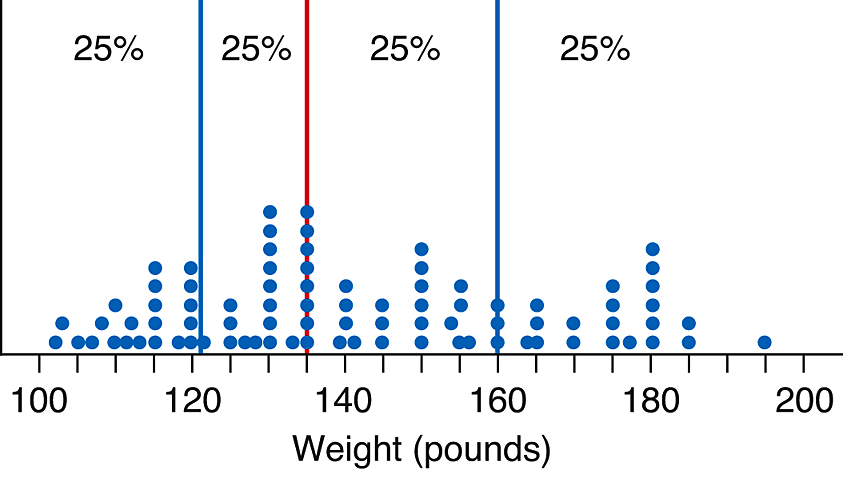
\includegraphics[width=0.7\linewidth]{images/math211_figure_3p18}
  \end{center}
  \pagebreak
  
  \begin{ex*}[Computing quartiles by hand]
    A group of eight children have the following heights (in inches):
    
    \noindent
    \begin{minipage}{0.4\linewidth}
      \[14, 10, 20, 20, 40, 20, 10, 10, 20, 50, 10\]
    \end{minipage}
    \hspace*{\stretch{1}}%
    \begin{minipage}{0.575\linewidth}
      \centering
      \begin{tikzpicture}
        \begin{axis}[
          axis lines=center,
          axis line style={black,->},
          xmin=44, xmax=74,
          ymin=0, ymax=4,
          ymajorticks=false,
          width=\linewidth,
          height=0.33\linewidth,
          ticklabel style={font=\normalsize,inner sep=0.5pt,fill=white,opacity=1.0, text opacity=1}]
          \foreach \price/\freq in {
            48/2,
            53/1,
            53.5/1,
            54/1,
            60/1,
            62/1,
            71/1
            }{
            \foreach \x in {1,...,\freq}
              \addplot[soldot, mark size=2pt] coordinates{(\price,\x)};
            }
        \end{axis}
      \end{tikzpicture}
    \end{minipage}
    \vspace*{\baselineskip}
    
    \noindent
    Find the following:
    \begin{tasks}[after-item-skip=\stretch{1}, label=\textbullet](1)
      \task The median, which is also referred to as Q2
      \task The first quartile (Q1), which is the median of the lower half of the sorted data
      \task The third quartile (Q3), which is the median of the upper half of the sorted data
      \task Compute the IQR
    \end{tasks}
    \vspace*{\stretch{1}}
  \end{ex*}

  \pagebreak
\end{document}
